\chapter{Definiciones y acornimos}
\label{Appendix:1}

\chapterquote{Saber dónde encontrar la información y cómo usarla. Ese es el secreto del éxito} {Albert Einstein}
-

Dedicaremos este apéndice a la explicación de conceptos en mas extensión, ya sea conceptos mas generales o la explicación del significado de los Acronimos de esta memoria.

\subsection{Definiciones}

Separaremos este apartado, de la misma manera que se ha hecho en otras partes de la memoria, en los tres grandes elementos que conforman esta memoria, definiciones referentes a datos, a nubes y a Inteligencia artificial.

\subsubsection{Referente a datos}

\begin{enumerate}
	\item El gobierno de España define los \textbf{datos de alto valor} \label{def1}  como “documentos cuya reutilización está asociada a considerables beneficios para la sociedad, el medio ambiente y la economía, en particular debido a su idoneidad para la creación de servicios de valor añadido, aplicaciones y puestos de trabajo nuevos, dignos y de calidad, y al número de beneficiarios potenciales de los servicios de valor añadido y aplicaciones basados en tales conjuntos de datos” Esta definición nos ofrece varias pistas sobre la manera en la que se prevé que se identifiquen esos conjuntos de datos de alto valor a través de una serie de indicadores que incluirían:
		\begin{itemize}
			\item Su potencial para generar beneficios sociales o medioambientales significativos.
			
			\item Su potencial para generar beneficios económicos y nuevos ingresos.
			
			\item Su potencial para generar servicios innovadores.
			
			\item Su potencial en cuanto a número de usuarios beneficiados, con atención particular a las PYMEs.
			
			\item Su capacidad para ser combinados con otros conjuntos de datos
		\end{itemize}
		
	\item El \textbf{open government} \label{def2} o gobierno abierto es una forma de comunicación abierta, permanente y bidireccional entre la administración y los ciudadanos, basada en la transparencia por parte de la administración y la participación y colaboración con la sociedad civil y las empresas. Teniendo como punto clave el movimiento open data o datos abiertos, esta estructura y formatos abiertos permiten que los datos puedan reutilizarse proporcionando nuevos servicios a ciudadanos y empresas. En Europa sus orígenes se sitúan en la Directiva 2003/98/CE del Parlamento y del Consejo Europeos sobre el acceso y la reutilización de la información del sector público. \citep{OperGovernment2011}
	
	\item El \textbf{Valor Público} se puede definir de muchas maneras y depende de la perspectiva de muchos autores:
	\label{def3} 
	\begin{itemize}
		\item[\textbullet] Para \textbf{Mark Moore}, su creador, consiste en conocer y satisfacer los deseos de la gente, un valor que lo público debe crear de forma análoga a como el sector privado crea valor económico. \citep{moore1995creating}
		\item[\textbullet] \textbf{Bozeman} lo define desde una perspectiva ciudadana como el consenso sobre los derechos y obligaciones de los ciudadanos, asi como los principios sobre los que debe basarse el gobierno  \citep{bozeman2007public}. A menudo se refiere a ``valores públicos'', en plural, para destacar su diversidad, tema que seria llevado mas en profundidad por \textbf{Talbot}, que sugiere que a veces estos son contradictorios entre sí, reflejando la combinación de las diversas y conflictivas preferencias del público \citep{Talbot01012011}.
		\item[\textbullet] \textbf{Benington} lo vincula directamente con la ``esfera pública'', argumentando que el valor público no es solo lo que el público valora individualmente, sino también aquello que agrega valor a este espacio colectivo. \citep{Benington19032009}
		\item[\textbullet] Finalmente, \textbf{Timo Meynhardt} lo conceptualiza como un fenómeno relacional que surge de las percepciones. El valor público se crea en la relación entre el individuo y la sociedad, y depende de cómo las acciones de las organizaciones públicas impactan en la satisfacción de las necesidades básicas de las personas: morales, sociales, utilitarias y hedonistas  \citep{Meynhardt19032009}.
	\end{itemize}
	
	En un intento de resumirlo, el valor publico surge de las evaluaciones y percepciones que los individuos y colectivos realizan sobre cómo las acciones, servicios o políticas de las organizaciones públicas (y otras entidades) impactan en la satisfacción de sus diversas necesidades básicas dentro de un marco relacional que involucra a la esfera pública. Valor creado para y por la sociedad.


	\item Los \textbf{Datos Abiertos} \label{def4} se refieren a conjuntos de datos digitales que se publican bajo una filosofía de apertura, garantizando y facilitando el libre acceso, uso, modificación, reutilización y redistribución por parte de cualquier persona o entidad, en cualquier momento, lugar y con cualquier finalidad. Una parte especifica y importante para este trabajo son los Datos Abiertos de Gobierno, aquellos datos que se originan, producen, encargan o publican los gobiernos u organismos públicos en el ejercicio de sus funciones. Estos datos buscan, como fin último, fomentar la transparencia, la creación de valor público, la colaboración intersectorial y la resolución de problemas.
	
	La materialización de esta filosofía de apertura se concreta en requisitos técnicos y jurídicos específicos, cuya interpretación puede variar ligeramente entre las entidades que los definen. Desde el Grupo de Trabajo sobre Datos Abiertos ``Open Knowledge Foundation'' (OKF), “El conocimiento está abierto si alguien tiene la libertad de acceder a él, usarlo, modificarlo y compartirlo, sujeto, como máximo, a medidas que preserven su procedencia y su apertura” \citep{OpenKnowledgeFoundation}. El Portal Europeo de Datos y el ``Open Data Charter'', por su parte, enfatizan las condiciones de acceso y las libertades de uso, incluyendo la gratuidad y la ausencia de limitaciones, detallando la necesidad de características técnicas y jurídicas para que los datos sean libremente reutilizables y redistribuibles \citep{dataEuropaOpenData}, \citep{Open_Data_Charter}.
	Todo esto subraya la complejidad y la multifuncionalidad de los Datos abiertos como catalizador para la innovación y el desarrollo socioeconómico, con implicaciones legales y técnicas que deben ser gestionadas cuidadosamente para maximizar su potencial.
	
	\item Las \textbf{Tres olas del ``Open Data'' } \label{def5} representan las diferentes etapas evolutivas por las que ha transitado el movimiento de apertura de datos. 
	La \textbf{Primera Ola} (1990s-2000s) se fundamentó principalmente en Estados Unidos, dirigido a periodistas, abogados y activistas que solicitaban datos específicos bajo el modelo de ``derecho a saber'', enfrentando riesgos de secretismo gubernamental y requiriendo auditores de información. 
	La \textbf{Segunda Ola} (2000s-2010s) evolucionó hacia la apertura por defecto con alcance internacional, expandiendo su audiencia a agencias gubernamentales, empresas tecnológicas y organizaciones comunitarias,pero generando desafíos de privacidad que impulsaron la creación de portales de datos abiertos y responsables.
	La \textbf{Tercera Ola} (2010s-presente) representa la madurez del movimiento  con colaboración intersectorial y flujos transfronterizos, dirigiéndose a ONGs, instituciones académicas, pequeñas empresas y gobiernos, estableciendo marcos de responsabilidad en materia de datos. 
	Esta evolución se visualiza en la siguiente tabla comparativa:
	
	\begin{table}[ht]
		\centering
		\caption{Resumen de las principales características de las denominadas olas de datos abiertos.}
		\label{tab:olas_datos_abiertos}
		\resizebox{\textwidth}{!}{
			\begin{tabular}{|p{3cm}|p{4cm}|p{4cm}|p{5cm}|}
				\hline
				\textbf{} & \textbf{Primera ola} & \textbf{Segunda ola} & \textbf{Tercera ola emergente} \\
				\hline
				\textbf{Concepto} & Libertad de información & Datos públicos abiertos & Reutilización de datos públicos y privados \\
				\hline
				\textbf{Propuesta de valor} & Transparencia & Transparencia y resolución de problemas & 
				\begin{itemize}
					\item Elaboración de políticas basadas en pruebas
					\item Innovación e iniciativa empresarial
				\end{itemize} \\
				\hline
				\textbf{Método} & Datos a petición (derecho a saber) & Abierto por defecto (derecho a compartir) & Publicar con propósito \\
				\hline
				\textbf{Enfoque} & Enfoque de impulso & Enfoque de atracción & Asociaciones (colaboraciones con datos) \\
				\hline
				\textbf{Énfasis geográfico} & Nacional & Internacional y nacional & 
				\begin{itemize}
					\item Subnacional y local
					\item Flujo transfronterizo de datos con fines específicos
				\end{itemize} \\
				\hline
				\textbf{Audiencia / Demanda} & 
				\begin{itemize}
					\item Periodistas
					\item Abogados y activistas
					\item Tecnólogos cívicos y ``data geeks''
				\end{itemize}
				& 
				\begin{itemize}
					\item Agencias gubernamentales
					\item Empresas, start-up tecnológicas
					\item Organizaciones comunitarias
				\end{itemize}
				& 
				\begin{itemize}
					\item ONG, derechos humanos y justicia social
					\item Instituciones académicas
					\item Pequeñas empresas y start-ups
					\item Gobierno
				\end{itemize} \\
				\hline
				\textbf{Riesgos y políticas} & Secretismos y ofuscación & Privacidad -- Efecto mosaico, información demográfica identificable (DII) & Marco de responsabilidad y derechos en materia de datos \\
				\hline
				\textbf{Respuestas institucionales} & Auditores de información & 
				\begin{itemize}
					\item Responsable de datos
					\item Portales de datos abiertos
				\end{itemize}
				& 
				\begin{itemize}
					\item Director de datos
					\item Intermediarios
				\end{itemize} \\
				\hline
			\end{tabular}
		}
		\vspace{0.5em}
		
		\footnotesize Fuente: Traducción propia de \cite{verhulst2020}.
	\end{table}

	\item La \textbf{Teoría de la Ventana} \label{def6} \citep{Matheus03052020} es un marco conceptual que analiza la transparencia generada por los Datos Abiertos de Gobierno, concibiéndola como una ``ventana'' que el gobierno abre para que el público vea su funcionamiento interno. Postulando que la transparencia es una construcción diversa y continua, cuyo objetivo principal es facilitar la transferencia de información entre el gobierno y sus públicos. Su materialización está influenciada por factores que la facilitan o impiden, clasificados en características de los datos, del sistema, de la organización y del uso individual, y genera consecuencias intencionadas o no, como la rendición de cuentas, la participación cívica, la eficiencia o la afectación a la privacidad.
	
	\item Un \textbf{``Datathon''} \label{def7} \citep{Datathon2016Anslow} es un evento colaborativo o competitivo intensivo centrado en datos, y derivado de los términos ``data'' y ``maratón'', donde equipos de expertos y otros individuos se reúnen para analizar grandes volúmenes de estos datos con el fin de encontrar soluciones innovadoras a problemas específicos. Esto va desde desarrollar aplicaciones para sacar partido a estos datos, hasta la optimización de procesos o la creación de modelos predictivos, las posibilidades son amplias.
	
	
	\newpage
	
	
	\subsubsection{Referente a Cloud}
	
	\item La \textbf{``Computación distribuida'' / ``Nube distribuida''} \label{def8} es un paradigma que aprovecha la capacidad de cálculo de miles o millones de dispositivos conectados a internet, creando una red de computación masiva, paralela y descentralizada. Los usuarios solo necesitan instalar un cliente de software que, cuando su dispositivo no está en uso, se encarga de descargar un pequeño fragmento de datos, procesarlo y devolver el resultado a un servidor central que coordina todas las tareas y ensambla los resultados finales. Este es un enfoque especialmente adecuado para problemas altamente paralelizables. Uno de los primeros productos en llevar la idea a cabo fue BOINC \citep{Anderson2004BOINC} para ayudar al cómputo de proyectos científicos. Actualmente, nubes como AWS o GCP se han apropiado del termino Nube distribuida, teniendo centros de datos en diferentes localizaciones para distribuir su trabajo a localizaciones mas cercanas o llevar la propia infraestructura y servicios de la nube fuera de sus data centres \citep{distributedGCP}.
	Esta idea evolucionó hasta la llamada ``Computación Voluntaria'' \citep{Anderson2010Volunteer}, donde dispositivos personales de voluntarios se usaban para este fin (ahora BOINC, cuyo software aún está disponible seria considerado computación voluntaria), y también se puede considerar que este paradigma se usa de forma malintencionada con varios casos famosos de ataques DDoS distribuidos \citep{MydoomDDoSMalware}, \citep{12Botnets} que usan dispositivos infectados para conseguir su propósito.
	
	También han surgido modelos con estas ideas paradigmas como el ``Dew computing'' \citep{DewComputing2018} donde los dispositivos personales se usan como almacenamiento, o plataformas de ``fog computing'' (que añade dispositivos intermedios en el calculo centralizado) o ``edge computing'' (Que ejecuta directamente en dispositivos finales) como SONM \citep{SONMWhitepaper} o otros proyectos \citep{BlockchainBasedDecentralisedCloud2018} que surgieron con el auge de las ``Blockchains'' y las usaban para poner en contacto usuarios que quisieran proporcionar potencia de cálculo con quienes querían usarla. En la actualidad, hay nubes que siguen activas como \citep{GolemNetwork}, \citep{akashCloud} ó \citep{rendernetwork}
	
	En resumen, todo lo englobado a la computación distribuida que hemos comentado se puede ver en esta tabla:
	
	\begin{table}[!tbp]
		\centering
		\begin{tabular}{|p{0.15\textwidth}|p{0.55\textwidth}|p{0.30\textwidth}|}
			\hline
			\textbf{Modelo} & \textbf{Descripción} & \textbf{Ejemplo destacado} \\ \hline
			Nube distribuida & Infraestructura descentralizada, extendiendo servicios hacia el edge o centros locales. & Gestión centralizada con despliegue en edge/localización (AWS CloudFront, Google Cloud CDN). \\ \hline
			Computación voluntaria & Uso de recursos ociosos de dispositivos personales para cómputo distribuido voluntario. & BOINC, SETI@home, HTCondor, Techila Grid. \\ \hline
			``Dew Computing'' & Combina almacenamiento local y en la nube, sincronizando datos y permitiendo disponibilidad offline. & Dropbox. \\ \hline
			``Fog Computing'' & Procesamiento intermedio entre dispositivos y la nube, reduciendo latencia y uso de ancho de banda. & Aplicaciones IoT y casos de baja latencia / Vehículos autónomos. \\ \hline
			``Edge Computing'' & Procesamiento en dispositivos finales, priorizando latencia y seguridad. & Procesamiento de vídeo en tiempo real, reconocimiento facial en dispositivos móviles. \\ \hline
			``BotNets'' & Redes de dispositivos comprometidos que realizan tareas maliciosas de forma distribuida, usando el mismo principio de cómputo compartido pero con fines ilícitos. & Ataques DDoS (Mydoom), spam masivo, minería de criptomonedas no autorizada. \\ \hline
		\end{tabular}
		\caption{Comparación de modelos relacionados con la computación distribuida.}
		\label{tab:nube_distribuida}
	\end{table}
	
	\newpage %[TODO] revisar si quitar al final
	
	\item La \textbf{clasificación de la Computación en Nube} \label{def9} típicamente se puede dividir según dos dimensiones principales \citep{huawei2023cloud}:
	
	\textbf{Por modelo de operación:}
		\begin{itemize}
			\item \textbf{Nube Pública:} Infraestructura compartida y gestionada por proveedores externos (ej. AWS, Azure, Google Cloud), la cual ofrece acceso universal mediante pago por uso.
			\item \textbf{Nube Privada:} Infraestructura exclusiva para una organización, gestionada interna o externamente, y que tiene mayor control y seguridad.
			\item \textbf{Nube Comunitaria:} Compartida por varias organizaciones con intereses comunes (ej. instituciones académicas), y que presenta un equilibrio entre control y costes.
			\item \textbf{Nube Híbrida:} Combina nubes públicas y privadas, permitiendo mover cargas de trabajo según necesidades de seguridad, coste o escalabilidad.
			\item \textbf{Nube Industrial:} Especializada en sectores específicos (sanidad, automoción), con componentes optimizados para casos de uso particulares.
		\end{itemize}
		
		\textbf{Por modelo de servicio:}
		\begin{itemize}
			\item \textbf{IaaS (Infraestructura como Servicio):} Proporciona recursos fundamentales (máquinas virtuales, almacenamiento, redes). Ej: Amazon EC2, Google Compute Engine.
			\item \textbf{PaaS (Plataforma como Servicio):} Ofrece entornos de desarrollo y ejecución para aplicaciones. Ej: Google App Engine, Microsoft Azure App Services.
			\item \textbf{SaaS (Software como Servicio):} Software completo gestionado por el proveedor y accesible vía web. Ej: Gmail, Salesforce, Office 365.
		\end{itemize}
		
		\begin{figure}[!tbp]
			\begin{center}
				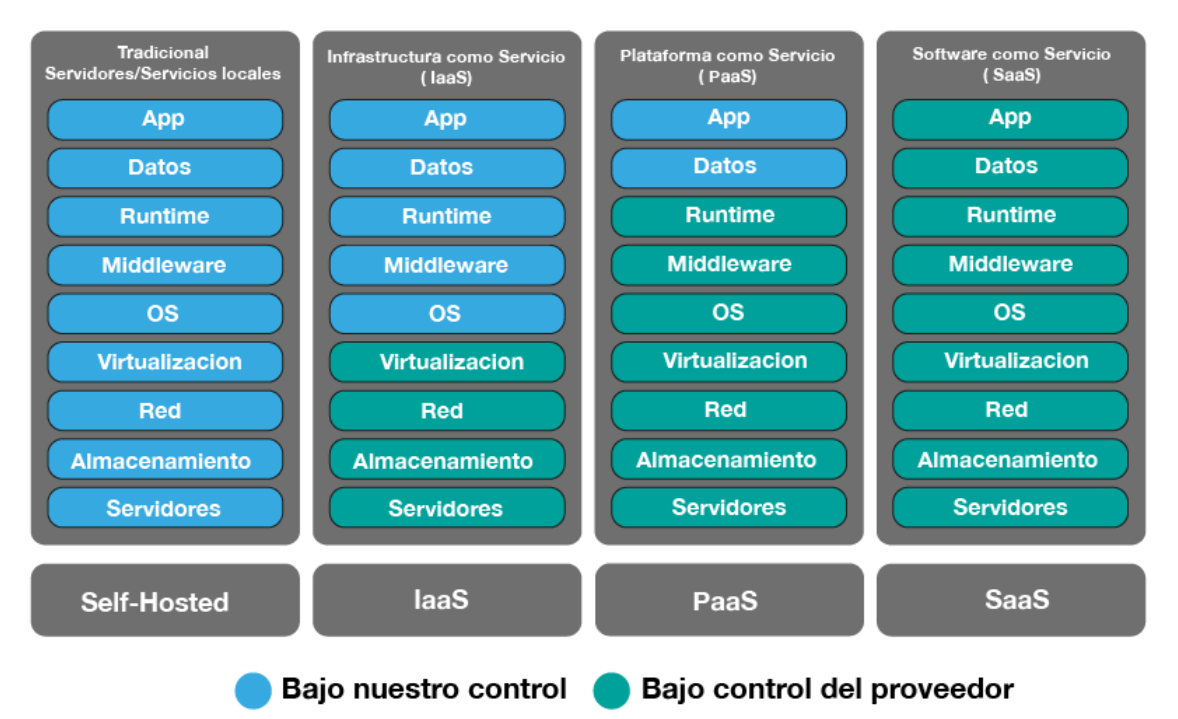
\includegraphics[scale=0.5]{Imagenes/Bitmap/distintos_tipos_clouds.png} 
				\caption{Distintos tipos de cloud, fuente: \citep{cloudPizza2014}.}
			\end{center}
		\end{figure}
		
			
		
		\newpage
		
		
	\subsubsection{Referente a Inteligencia Artificial}
		
		
		
\end{enumerate}




\newpage

\subsection{Acronimos}
\label{sec:acronimos}

\begin{description}
	
	\item[AI] Inteligencia Artificial (Artificial Intelligence)
	\item[API] Interfaz de Programación de Aplicaciones (Application Programming Interface)
	\item[AWS] Amazon Web Services
	\item[BOINC] Berkeley Open Infrastructure for Network Computing
	\item[CCPA] Ley de Privacidad del Consumidor de California (California Consumer Privacy Act)
	\item[CDN] Red de Distribución de Contenidos (Content Delivery Network)
	\item[CNMC] Comisión Nacional de los Mercados y la Competencia
	\item[CPU] Unidad Central de Procesamiento (Central Processing Unit)
	\item[CSV] Valores Separados por Comas (Comma-Separated Values)
	\item[D1] D1 Database (Base de datos de Cloudflare)
	\item[DDoS] Ataque de Denegación de Servicio Distribuido (Distributed Denial of Service)
	\item[DNS] Sistema de Nombres de Dominio (Domain Name System)
	\item[DSL] Ley de Seguridad de Datos (Data Security Law) - China
	\item[EEUU] Estados Unidos
	\item[EU] Unión Europea
	\item[GCP] Google Cloud Platform
	\item[GPU] Unidad de Procesamiento Gráfico (Graphics Processing Unit)
	\item[HIPAA] Ley de Portabilidad y Responsabilidad de Seguros de Salud (Health Insurance Portability and Accountability Act)
	\item[IBM] International Business Machines
	\item[INE] Instituto Nacional de Estadística
	\item[JSON] Notación de Objetos de JavaScript (JavaScript Object Notation)
	\item[KV] Key-Value (Almacenamiento Clave-Valor)
	\item[LGD] Ley de Gobernanza de Datos
	\item[ML] Aprendizaje Automático (Machine Learning)
	\item[MLOps] Operaciones de Aprendizaje Automático (Machine Learning Operations)
	\item[NLP] Procesamiento del Lenguaje Natural (Natural Language Processing)
	\item[OECD] Organización para la Cooperación y el Desarrollo Económicos
	\item[OGDA] Ley de Datos Abiertos del Gobierno (OPEN Government Data Act)
	\item[OCI] Oracle Cloud Infrastructure
	\item[PIPL] Ley de Protección de Información Personal (Personal Information Protection Law) - China
	\item[R2] R2 Storage (Almacenamiento de Cloudflare)
	\item[RAM] Memoria de Acceso Aleatorio (Random Access Memory)
	\item[RGPD] Reglamento General de Protección de Datos
	\item[SASE] Acceso Seguro al Borde del Servicio (Secure Access Service Edge)
	\item[SSL] Capa de Conexión Segura (Secure Sockets Layer)
	\item[SSD] Disco de Estado Sólido (Solid State Drive)
	\item[TPU] Unidad de Procesamiento Tensorial (Tensor Processing Unit)
	\item[TURN] Traversal Using Relays around NAT
	\item[UE] Unión Europea
	
\end{description}


 \newpage
